\chapter{Results}
\label{chap:res}
In this section we will present and discuss the results from the experiments on the REST implementation. The experiments were conducted on an Intel(R) Xeon(R) Gold 6426Y processor with 500 GB RAM.

\section{Reference Set Construction}
Firstly we will look at reference set construction, both in terms of performance and set size. The metrics \textit{Sample size} and \textit{Window size} is the sample size to construct the reference set and the square's side length in the range query in meters. A window size of 5 means a box of $5\times5m^2$ for r-tree queries. \textit{REST} is the implementation of the original algorithm, while \textit{REST-SF} is the same implementation with a spatial filter. The window size is also indicated in the name, following SF.

\begin{figure}[ht]
    \begin{minipage}[b]{0.49\linewidth}
        \centering
        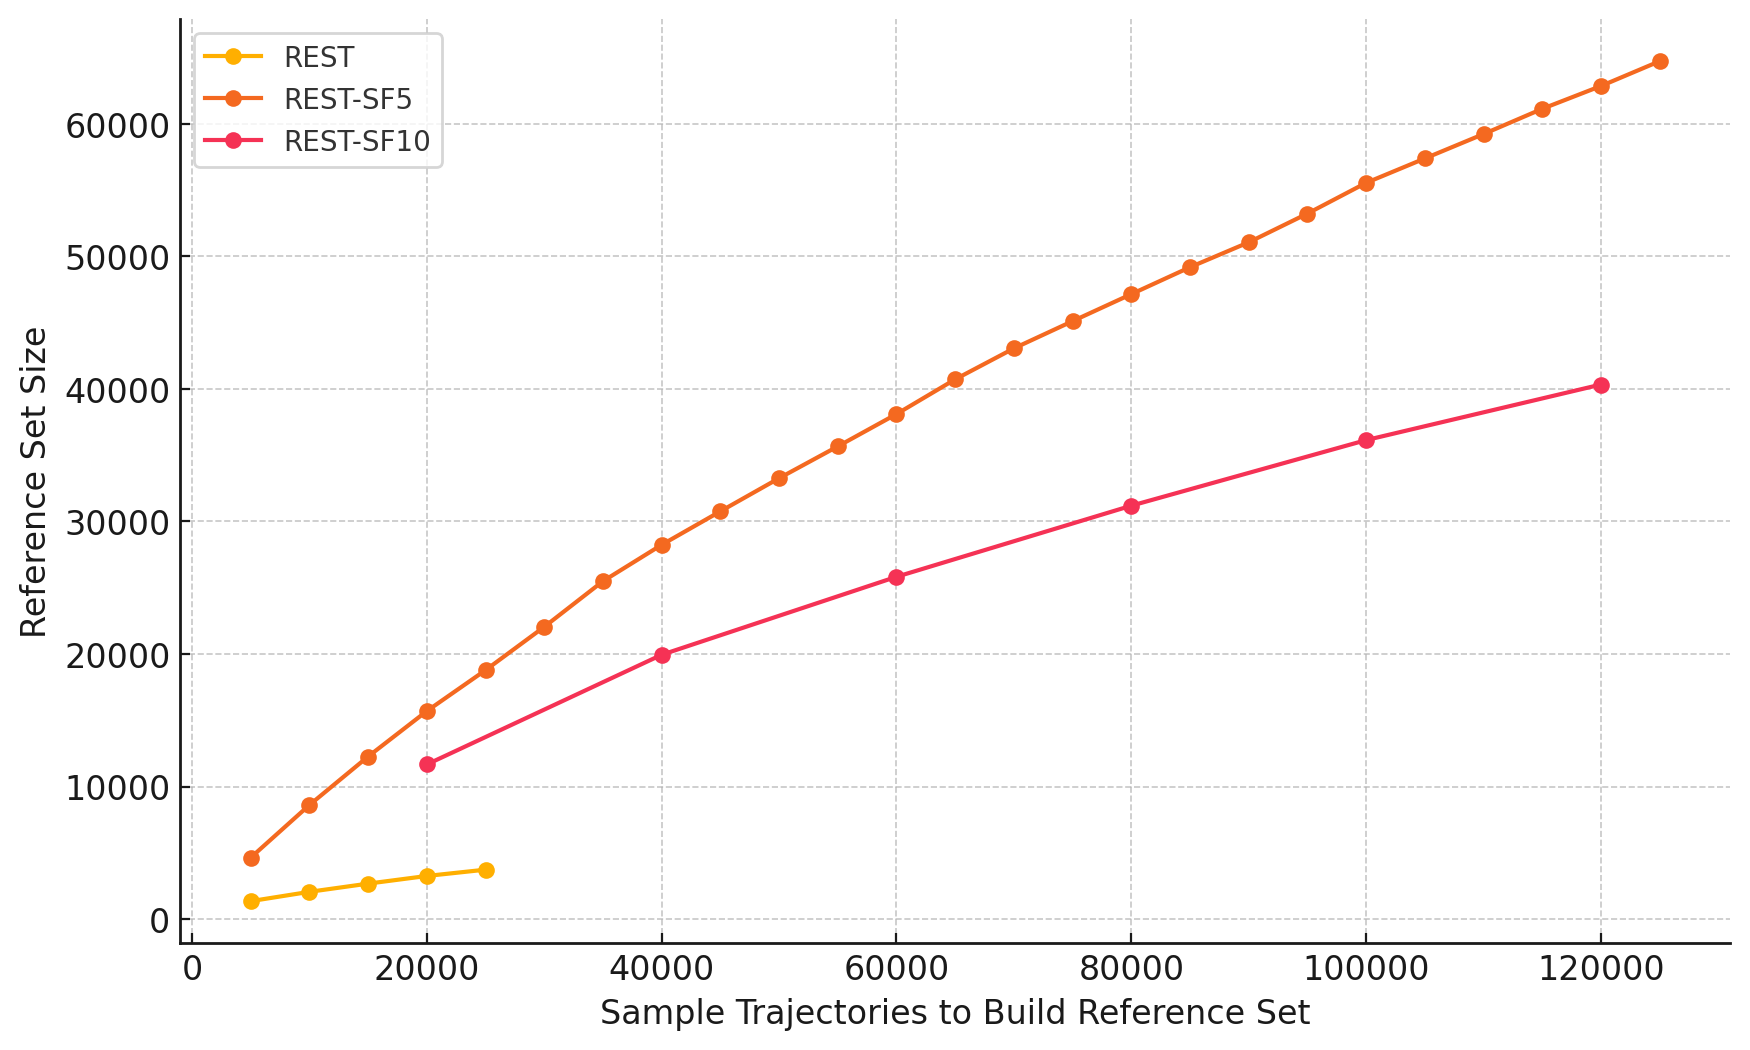
\includegraphics[width=\linewidth, height=7cm, keepaspectratio]{./figures/set_size.png}
        \caption{Reference Set Size by Sample Size}
        \label{fig:set_size}
    \end{minipage}
    \begin{minipage}[b]{0.49\linewidth}
        \centering
        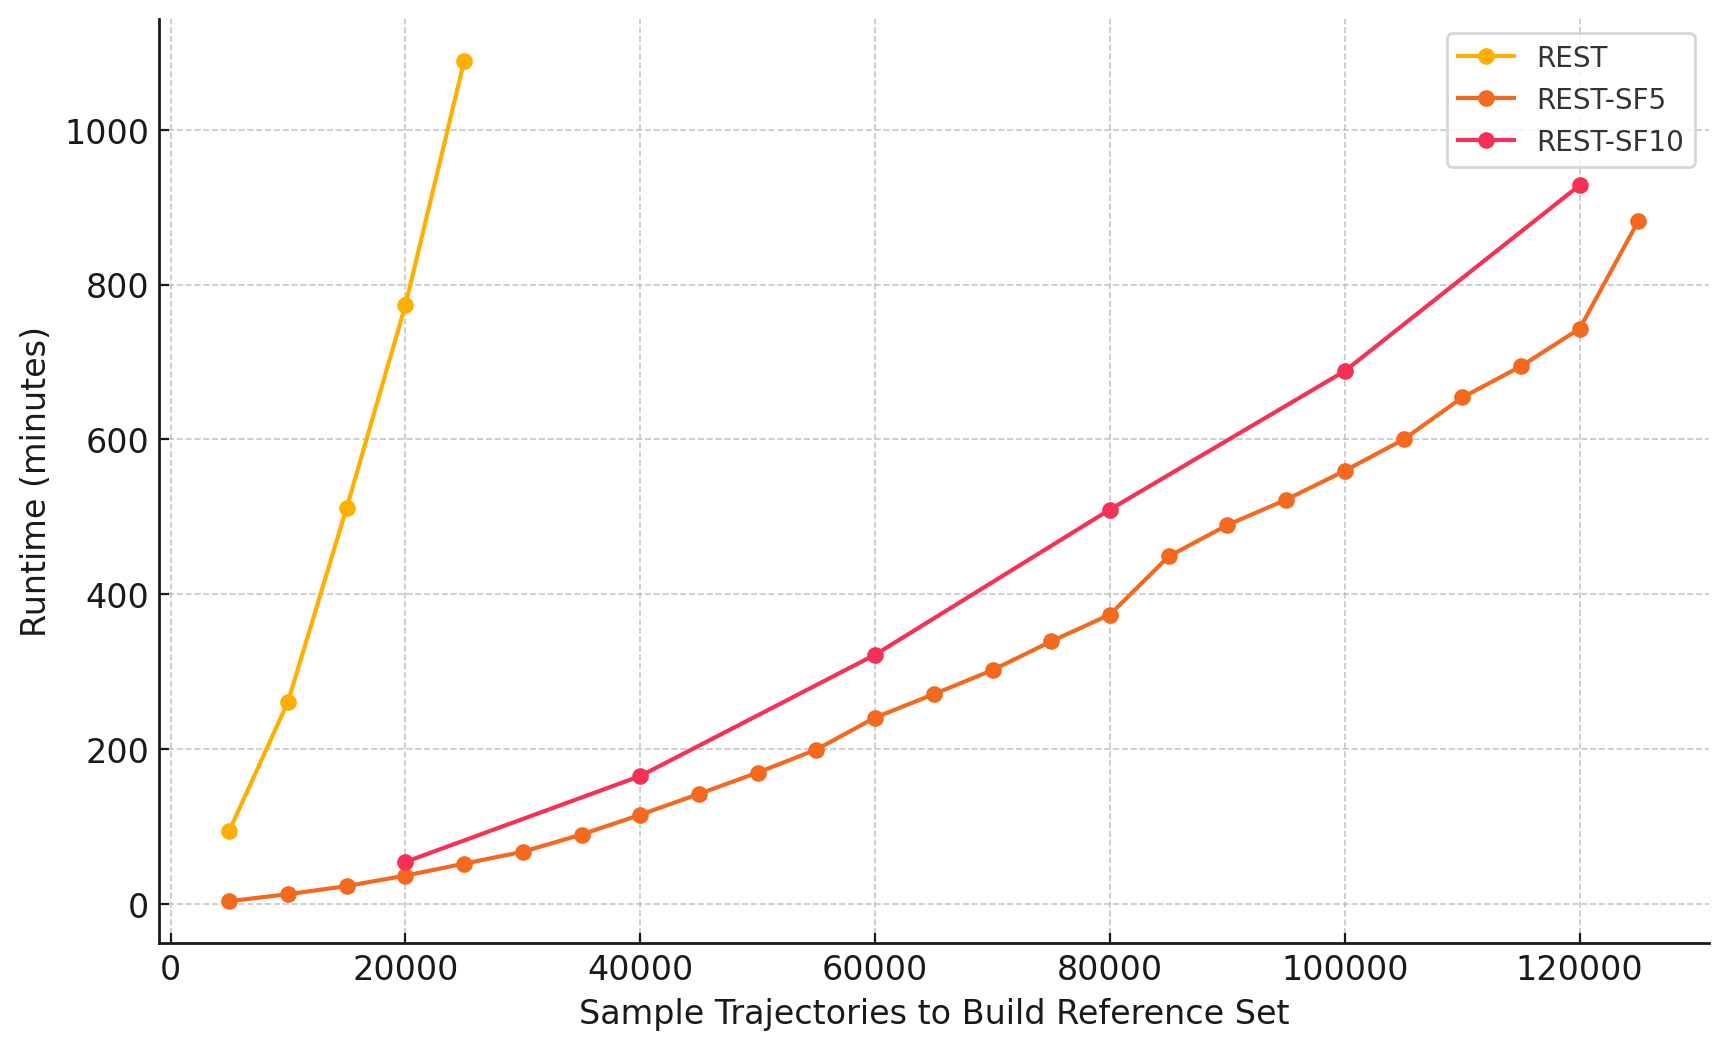
\includegraphics[width=\linewidth, height=7cm, keepaspectratio]{./figures/set_runtime.png}
        \caption{Reference Set Construction runtime by Sample Size}
        \label{fig:set_runtime}
    \end{minipage}
\end{figure}

In figure \ref{fig:set_size} we can see that \textit{REST} has a very low set size to sample size ratio, meaning it can represent a large sample with a small set. It is significantly lower than \textit{REST-SF5} and \textit{REST-SF10} (hopefully some larger window size will have a similar performance in this regard). We also see that for all variants there is some slowing of the growth. This might indicate there is some threshold where the reference set stops growing even as the sample size grows. This would mean that the reference set size converges. This convergance would also strongly depends on the data set frequency and precision. Moreover, if the value converges, it makes a strong case for the effectiveness of reference based compression strategies in general. Intuitively this can be seen as the road network of a given city. If all the roads / routes have been mapped by the reference set then all new routes can also be represented by that. Note however, that the road network is not mapped directly, but indirectly through the data itself while supporting an unconstrained space (unlike the PRESS algorithm).

For the runtime seen in \ref{fig:set_runtime} it is clear that \textit{REST} is much slower than the spatial filter variants. This is likely because \textit{REST-SF} only considers subtrajectories in proximity to the compressed trajectory. Even as the reference set size increases the range query selects a sufficiently small subset so that the runtime stays low. However, it seems to increase more near the end where $Sample Size = 120 000$.

\section{Compression Performance}
- Differnt distance measures, DTW and MaxDTW. Experiments for compression ratio and runtime.